\documentclass[11pt]{article}
% Font & ngôn ngữ tiếng Việt (pdfLaTeX)
\usepackage[utf8]{inputenc}
\usepackage[T5]{fontenc}			


% Biblatex + biber
\usepackage[backend=biber, style=alphabetic, sorting=ynt]{biblatex}
\addbibresource{references.bib}
\usepackage{listings}
\usepackage{xcolor}
\lstdefinestyle{shell}{
	language=bash,
	basicstyle=\ttfamily\small,
	commentstyle=\color{green!60!black},
	keywordstyle=\color{blue},
	stringstyle=\color{red},
	emphstyle=\color{purple},
	backgroundcolor=\color{gray!10},
	showstringspaces=false,
	frame=single,
	breaklines=true,
	emph={[1]\$\ },  % This is the key part: highlight the prompt
	emph=[1]{git, conda, mkdir, cd, pip} % Also emphasize key commands
}

% Toán học & font Times
\usepackage{amsmath, amssymb, amsfonts, bm}

% Bảng biểu & căn lề
\usepackage{longtable}
\usepackage{array}
\usepackage{booktabs}

% Đồ họa & màu sắc
\usepackage{graphicx}
\usepackage{xcolor}
\usepackage{float}
\usepackage{subcaption}

% Liên kết & tham chiếu
\usepackage{hyperref}
\hypersetup{
    colorlinks=true,
    linkcolor=blue,
    urlcolor=red,
    pdftitle={Overleaf Example},
    pdfpagemode=FullScreen,
}
\usepackage{bookmark}

% Dấu tick và x
\usepackage{pifont}
\newcommand{\xmark}{\ding{55}}
\newcommand{\cmark}{\ding{51}}

% Tiêu đề tùy chỉnh
\usepackage{titling}
\setlength{\droptitle}{-10em}
\renewcommand{\maketitle}{%
    \begin{center}
        \fontsize{18}{20}\selectfont\textbf{Data Version Control (DVC) \\[0.2em] in Machine Learning Projects}\\[1em]
        \fontsize{14}{16}\selectfont Nhóm MLOps\\[0.5em]
        \fontsize{14}{16}\selectfont Ngày 18 tháng 10 năm 2025
    \end{center}
    \vspace{1.5em}
}

% Format section (không đánh số)
\usepackage{titlesec}
\titleformat{\section}{\normalfont\Large\bfseries}{}{0em}{}

% Code block
\usepackage{listings}
\definecolor{backcolour}{rgb}{0.95,0.95,0.92}
\lstset{
    backgroundcolor=\color{backcolour},
    basicstyle=\ttfamily\footnotesize,
    breaklines=true,
    numbers=left,
    numberstyle=\tiny\color{gray},
    captionpos=b
}

% Hộp màu
\usepackage[many]{tcolorbox}
\definecolor{lightgreenbox}{rgb}{0.85,0.95,0.85}
\newtcolorbox{summarybox}{
    colback=lightgreenbox,
    colframe=green!50!black,
    boxsep=5pt, arc=4pt,
    boxrule=0.5pt,
    left=10pt, right=10pt,
    top=10pt, bottom=10pt,
}


% Layout trang
\setlength{\topmargin}{-0.7in}
\setlength{\textheight}{9.25in}
\setlength{\oddsidemargin}{0in}
\setlength{\textwidth}{6.8in}

%%%%%%%%%%%%%%%%%%%%%%%%%%%%%%%%%%%%%%%%%%%%%%%%%%%%%%%%%%%%%%%%%%%%%%%%%%%%%
\begin{document}

\maketitle

\begin{summarybox}
Nội dung về được chia thành 5 phần chính:
    \begin{itemize}
	\item \textbf{Revision: Data Versioning và ETL pipeline}
	\item \textbf{Overview: Giới thiệu vòng đời của 1 dự án Học Máy}
	\item \textbf{Feature Store và Feast là gì ?}
	\item \textbf{Case Study}
	\item \textbf{Final Revision: ôn lại mọi khái niệm trong bài cùng team Time Series}
    \end{itemize}
\end{summarybox}

% --- PHẦN 1 ---
\section{Phần 1: Từ ETL, Processing, Data Versoning đến Feature Store}
Hành trình của dữ liệu bắt đầu từ quy trình \textbf{ETL (Extract, Transform, Load)}. Đây là bước nền tảng giúp thu thập, chuẩn hóa dữ liệu thô từ nhiều nguồn đa dạng (như các CSDL, Excel, Ảnh, etc..), sau đó làm sạch, biến đổi và lưu trữ chúng vào một trung tâm tập trung như Data Warehouse.
\begin{figure}[H]
    \centering
    \includegraphics[width=0.8\linewidth]{images/etl.png}
    \caption{ETL pipeline}
\end{figure}

Giai đoạn tiếp theo là \textbf{Processing (Xử lý)}. Chúng ta không chỉ xử lý dữ liệu "tĩnh" (static) mà còn cả dữ liệu "động" (streaming data) như đơn hàng Shopee hay tin nhắn. Các công cụ như Apache Spark cho phép chúng ta xử lý và \textit{tạo ra các đặc trưng (features)} từ dữ liệu lịch sử (ví dụ: "số tiền chi tiêu trung bình của khách hàng X trong 30 ngày qua"). Đây là các đặc trưng dùng để \textbf{huấn luyện (training)} mô hình.

Chính tại đây, thách thức lớn đầu tiên xuất hiện. Khi mô hình được huấn luyện bằng các đặc trưng offline được tải về để huấn luyện này (ví dụ: "số tiền trung bình 30 ngày" được tính 1 lần/ngày bằng Spark), làm thế nào để khi mô hình được \textbf{dự đoán (inference)} trong thời gian thực, nó có thể nhận được \textit{chính xác} các đặc trưng đó (ví dụ: "số tiền trung bình 30 ngày" được tính ngay tại thời điểm 3:05:10 PM) ? \\

Hai quy trình này—một cho training (xử lý theo lô, offline) và một cho inference (xử lý thời gian thực, online)—thường được xây dựng độc lập. Điều này tất yếu dẫn đến hiện tượng \textbf{Training-Serving Skew}: dữ liệu mà mô hình "thấy" lúc huấn luyện khác với dữ liệu nó "thấy" lúc dự đoán.

\begin{figure}[H]
    \centering
    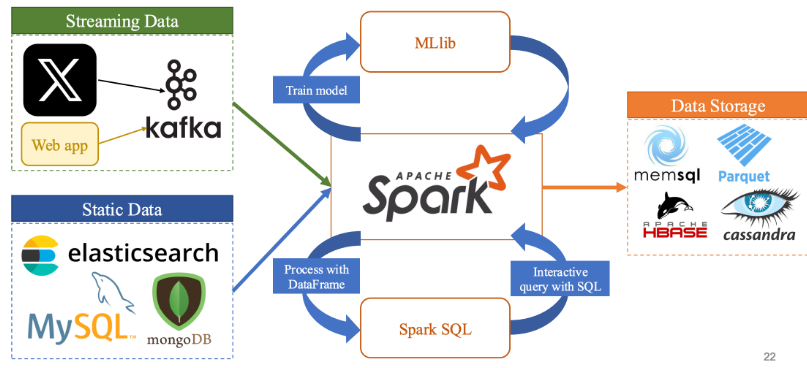
\includegraphics[width=0.8\linewidth]{images/proces.png}
    \caption{Process pipeline - Nơi bắt đầu xảy ra sự phân tách giữa pipeline offline (training) và online (serving).}
\end{figure}

Khi các mô hình trở nên phức tạp, chúng ta cần đến \textbf{Data Versioning}. Công cụ này giúp quản lý các "tạo tác" (artifacts) của quy trình \textit{huấn luyện}, như phiên bản mô hình, tệp tham số, và các bộ dữ liệu đã được tạo ra. Nó đảm bảo khả năng tái lặp lại các thử nghiệm, tương tự như Git quản lý mã nguồn.

\begin{figure}[H]
    \centering
    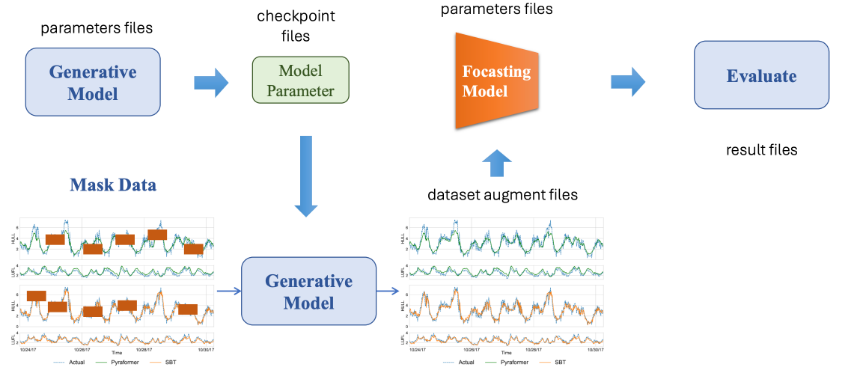
\includegraphics[width=0.8\linewidth]{images/dt_ver.png}
    \caption{Data versioning Pipeline}
\end{figure}

Cuối cùng, chúng ta có một bức tranh rõ ràng:
\begin{enumerate}
    \item \textbf{ETL} cung cấp dữ liệu thô.
    \item \textbf{Processing} (Spark) tạo ra các đặc trưng offline cho \textit{training}.
    \item \textbf{Data Versioning} (DVC) quản lý các phiên bản mô hình được tạo ra từ \textit{training}.
\end{enumerate}

Tuy nhiên, vẫn còn một "lỗ hổng" chí mạng: Làm thế nào để cung cấp các đặc trưng cho \textit{inference} (dự đoán) một cách nhất quán với các đặc trưng đã dùng để \textit{training}? Đây chính là bài toán mà \textbf{Feature Store} ra đời để giải quyết. Nó là cầu nối duy nhất, đảm bảo tính nhất quán của đặc trưng cho cả hai môi trường.


\section{Phần 2: ML/AI Project Lifecycle - Giới thiệu vòng đời của 1 dự án Học Máy}
Để dễ hình dung vòng đời của 1 dự án học máy gồm 4 giai đoạn, qua một ví dụ tuần tự: \textbf{Xây dựng một hệ thống phát hiện gian lạn thẻ tín dụng theo thời gian thực}:
\begin{itemize}
	\item \textbf{Data Engineering:} giải quyết vấn đề: \textit{"Chúng ta có dữ liệu gì ? có những kiểu, đặc điểm gì ? dùng nó để huấn luyện như thế nào ?"}. \\
 	  $\rightarrow$ Kỹ sư dữ liệu sẽ thu thập lịch sử giao dịch (dữ liệu tĩnh) từ Data Warehouse rồi làm sạch và biến đổi chúng để tạo ra các "đặc trưng" (features) như "số tiền chi tiêu trung bình của người dùng này trong 30 ngày qua" hay "số lần chuyển tiền trong 1 ngày > 20". Kết quả là một bộ dữ liệu sạch sẽ gồm những đặc trưng được kết hợp đại diện cho các yếu tố trong thực tế, sẵn sàng để huấn luyện.

	\item \textbf{Modeling:} giải quyết vấn đề: \textit{"Làm sao để tìm ra quy luật của các gian lận, những yêu tố, đặc trưng (feature) nổi bật của gian lận đó ?"}. \\
	 $\rightarrow$ Sau đó 1 nhóm gồm các Data Scientist sẽ nhận dữ liệu và huấn luyện các mô hình học máy hoặc học sâu, học các quy luật ngầm (patterns) đằng sau dữ liệu để phân biệt giữa 1 giao dịch bình thường và 1 giao dịch đáng ngờ (ví dụ: "số tiền lớn bất thường" + "vị trí lạ" $\rightarrow$ +"số lần chuyển tiền trong 1 ngày > 20" -> 95\% là gian lận).

	\item \textbf{Deployment:} giải quyết vấn đề: \textit{"Làm sao để ứng dụng (appication) dùng được mô hình này NGAY LẬP TỨC?"}. \\
	 $\rightarrow$ Khi đã có mô hình (ví dụ: file \texttt{model.pkl}), công việc triển khai không chỉ đơn giản là tải file này lên máy chủ. Thách thức lớn nhất là làm thế nào để \textbf{cung cấp dữ liệu đầu vào (features) cho mô hình} với tốc độ cực nhanh và phải \textit{nhất quán} với dữ liệu đã huấn luyện.
	Đây là lúc hiện tượng \textbf{Training-Serving Skew} thể hiện rõ ràng nhất qua các tình huống cụ thể:
	
	\begin{itemize}
	    \item \textbf{Tình huống 1: Sai lệch về Logic (Logic Skew).}
	    \begin{itemize}
	        \item \textit{Khi Training (Offline):} Nhà khoa học dữ liệu dùng Python/Pandas để tính đặc trưng "số lượng giao dịch trong 1 giờ qua". Khi tính, họ có thể dùng hàm \texttt{.fillna(0)} để điền số 0 vào những khoảng thời gian không có giao dịch.
	        \item \textit{Khi Serving (Online):} Kỹ sư phần mềm, để tối ưu tốc độ, có thể viết lại logic này bằng Java. Nhưng thay vì điền số 0, hệ thống online của họ lại \textit{bỏ qua} (ignore) các khoảng thời gian đó khi tính toán.
	        \item \textit{Kết quả:} Cùng một tên đặc trưng nhưng lại có hai giá trị khác nhau. Mô hình được huấn luyện với giá trị \texttt{0} nay lại nhận một giá trị khác, dẫn đến dự đoán sai.
	    \end{itemize}
	
	    \item \textbf{Tình huống 2: Sai lệch về Thời gian (Temporal Skew).}
	    \begin{itemize}
	        \item \textit{Khi Training (Offline):} Đặc trưng "số tiền chi tiêu trung bình 30 ngày" được tính theo lô (batch) và cập nhật vào lúc nửa đêm mỗi ngày.
	        \item \textit{Khi Serving (Online):} Một khách hàng thực hiện giao dịch lúc 3 giờ chiều. Hệ thống online lấy đặc trưng "số tiền trung bình 30 ngày" được cập nhật lúc nửa đêm (dữ liệu đã cũ 15 tiếng).
	        \item \textit{Kết quả:} Mô hình đang dự đoán dựa trên dữ liệu "cũ", trong khi lúc huấn luyện nó luôn được cung cấp dữ liệu "mới nhất" (tại thời điểm tính toán offline).
	    \end{itemize}
	
	    \item \textbf{Tình huống 3: Sai lệch về Giá trị Mặc định (Default Value Skew).}
	    \begin{itemize}
	        \item \textit{Khi Training (Offline):} Với một khách hàng mới chưa có giao dịch, script huấn luyện gán giá trị mặc định là \texttt{-1} cho đặc trưng "số tiền giao dịch cuối cùng".
	        \item \textit{Khi Serving (Online):} API phục vụ, khi không tìm thấy giao dịch cho khách hàng mới, lại trả về giá trị \texttt{null} hoặc \texttt{0}.
	        \item \textit{Kết quả:} Mô hình nhận được đầu vào mà nó chưa từng thấy trong quá trình huấn luyện, dẫn đến hành vi không đoán trước được.
	    \end{itemize}
	\end{itemize}
	
	Do đó, công việc của Kỹ sư AI trong giai đoạn này là phải tích hợp mô hình, tối ưu phần cứng (CPU, GPU, CUDA) và \textbf{quan trọng nhất} là đảm bảo pipeline dữ liệu đầu vào cho inference phải tuyệt đối nhất quán với pipeline dữ liệu đã dùng cho training.
	

	\item \textbf{Business Analysis \& Monitoring:} giải quyết vấn đề: \textit{"Mô hình có đang hoạt động đúng và mang lại giá trị không?"}.
	Cuối cùng, team phân tích kinh doanh sẽ giám sát để đánh giá hiệu quả của liệu mô hình có đáp ứng sát yêu cầu của doanh nghiệp hay không qua các thử nghiệm rồi báo cáo lại với team Data Engineer để đưa ra nhận định và cải tiến.

	Bốn giai đoạn này tạo thành một vòng lặp liên tục, và \textbf{AI Infrastructure (Cơ sở hạ tầng AI)} chính là nền móng (máy chủ, cơ sở dữ liệu, các công cụ) giúp toàn bộ vòng lặp này hoạt động một cách nhanh chóng, bảo mật và có thể mở rộng.
\end{itemize}

\noindent \textbf{Data Engineering}
\begin{figure}[H]
    \centering
    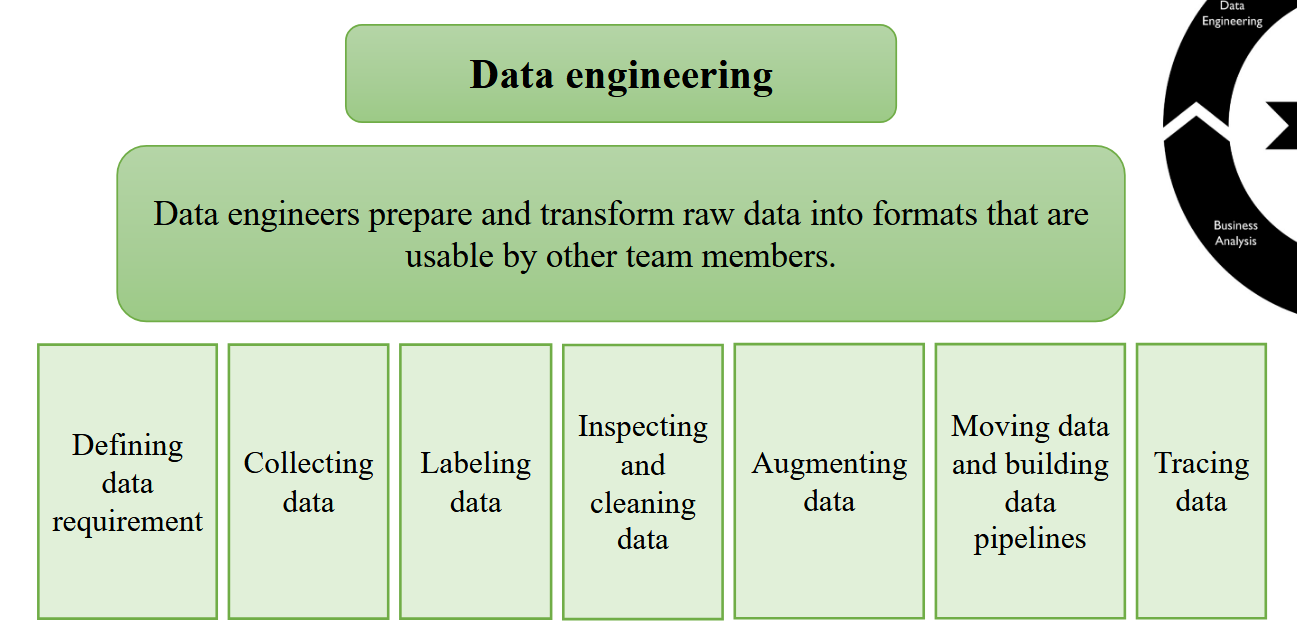
\includegraphics[width=0.8\linewidth]{images/dt_engineer.png}
    \caption{Data Engineer Pipeline}
\end{figure}
Trong ví dụ phát hiện gian lận, điều này có nghĩa là: \textbf{Defining data requirement} (định nghĩa dữ liệu giao dịch gồm những gì), \textbf{Collecting data} (thu thập dữ liệu từ hệ thống ngân hàng), \textbf{Inspecting and cleaning} (tìm và xử lý các giao dịch bị thiếu thông tin), và \textbf{Moving data and building data pipelines} (xây dựng quy trình tự động để các kiểu dữ liệu truyền qua đó trở thành dữ liệu sạch). \\

\noindent \textbf{Modeling}
\begin{figure}[H]
    \centering
    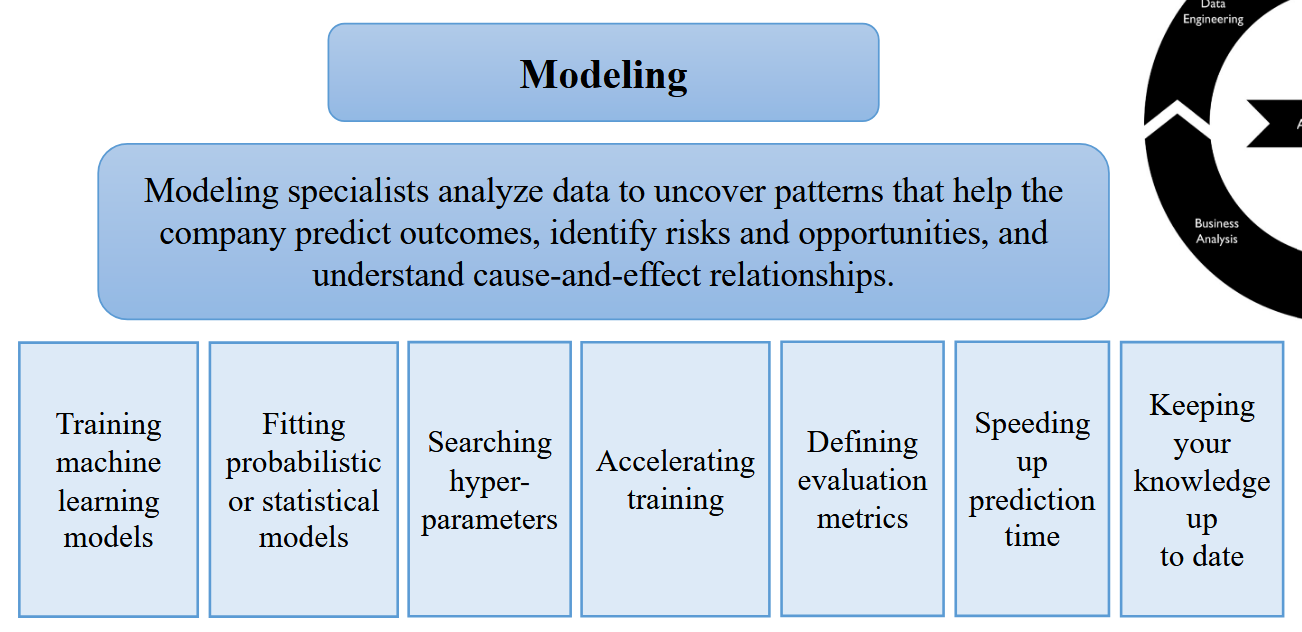
\includegraphics[width=0.8\linewidth]{images/modeling.png}
    \caption{Modeling ML Model Pipeline}
\end{figure}
Đối với các Data Scientist họ sẽ đảm nhiệm \textbf{Training machine learning models} (dạy mô hình phân biệt giao dịch thật/giả), \textbf{Searching hyper-parameters} (tinh chỉnh mô hình để nó hoạt động tốt nhất), và \textbf{Defining evaluation metrics} (quyết định dùng thước đo nào để cân bằng giữa Bias và Varianece, ví dụ: "thà chặn nhầm còn hơn bỏ sót gian lận"). \\

\noindent \textbf{Deployment}
\begin{figure}[H]
    \centering
    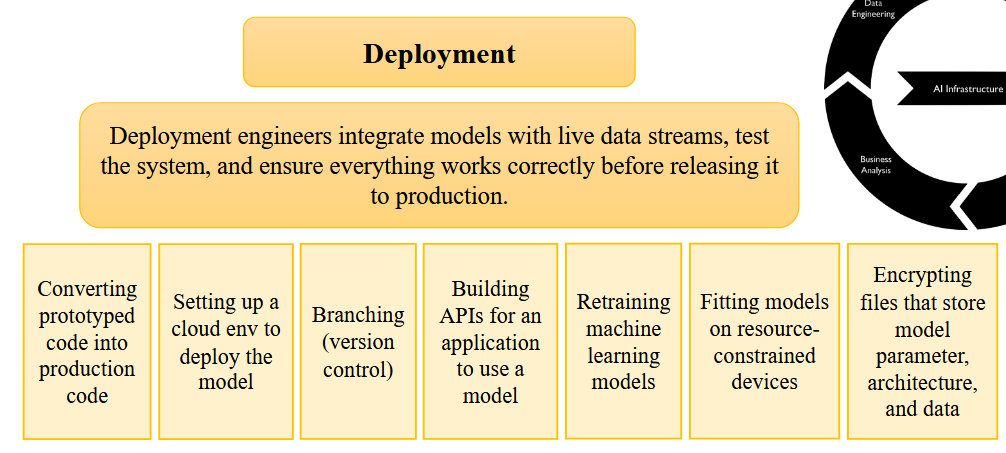
\includegraphics[width=0.8\linewidth]{images/deployment.png}
    \caption{ML Model Deplopyment Pipeline}
\end{figure}
Để đưa mô hình vào thực tế, Kỹ sư AI sẽ: \textbf{Converting prototyped code into production code} (chuyển code Python thử nghiệm thành code tối ưu, chạy nhanh), \textbf{Building APIs} (xây dựng API để tích hợp mô hình vào ứng dụng ngân hàng), và \textbf{Setting up a cloud env} (thiết lập máy chủ trên Cloud để mô hình chạy 24/7). \\

\noindent \textbf{Business analysis}
\begin{figure}[H]
    \centering
    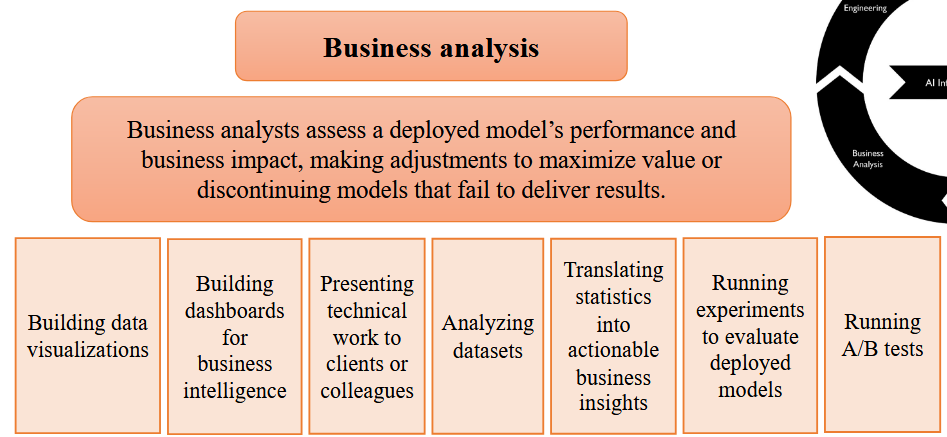
\includegraphics[width=0.8\linewidth]{images/business_analysis.png}
    \caption{Business Analysis Pipeline}
\end{figure}
Đối với team phân tích nghiệp vụ, họ sẽ: \textbf{Building data visualizations} và \textbf{dashboards} (tạo biểu đồ theo dõi tỷ lệ phát hiện gian lận), \textbf{Running A/B tests} (so sánh mô hình mới và mô hình cũ xem cái nào hiệu quả hơn), và \textbf{Translating statistics into actionable business insights} (dịch các con số kỹ thuật sang ngôn ngữ kinh doanh, ví dụ: "Mô hình mới đã tiết kiệm được 10 tỷ VNĐ trong tháng qua"). \\

\noindent \textbf{AI Infrastructure - Cơ sở hạ tầng của 1 dự án AI}
\begin{figure}[H]
    \centering
    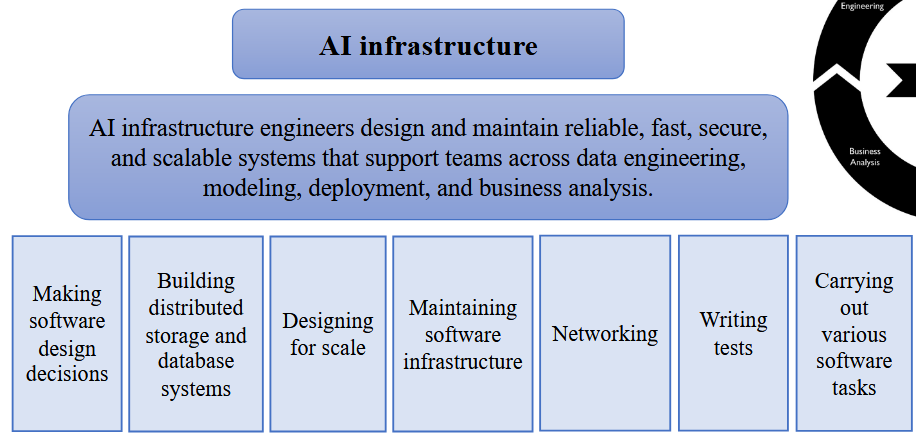
\includegraphics[width=0.8\linewidth]{images/ai_infra.png}
    \caption{AI Infrastructure Pipeline}
\end{figure}
Đây là \textbf{nền tảng} cho tất cả các giai đoạn trên. Để hệ thống gian lận hoạt động, đội ngũ hạ tầng phải: \textbf{Building distributed storage} (xây dựng CSDL có thể lưu trữ hàng tỷ giao dịch), \textbf{Designing for scale} (thiết kế để hệ thống không bị sập khi có hàng triệu người giao dịch cùng lúc), và \textbf{Maintaining software infrastructure} (bảo trì máy chủ, mạng...). \\

\noindent \textbf{6 vai trò trong nhóm phát triển AI} \\
Dựa trên các giai đoạn của vòng đời dự án, chúng ta có thể thấy 6 vai trò chính trong một nhóm AI và sự tham gia của họ vào các giai đoạn khác nhau. Sơ đồ dưới đây minh họa sự phân bổ trách nhiệm của từng vai trò:

\begin{figure}[H]
    \centering
    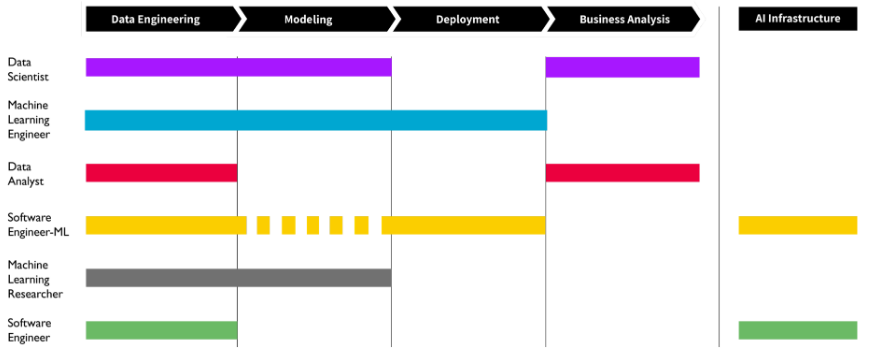
\includegraphics[width=0.8\linewidth]{images/aiteam.png}
    \caption{Sơ đồ phân bổ vai trò trong Vòng đời AI}
\end{figure}

\begin{itemize}
    \item \textbf{Data Scientist (Nhà khoa học dữ liệu):} Tham gia sâu vào \textbf{Data Engineering} (chuẩn bị, khám phá dữ liệu) và \textbf{Modeling} (xây dựng mô hình). Họ cũng đóng vai trò quan trọng trong giai đoạn \textbf{Business Analysis} để đánh giá kết quả và tác động kinh doanh.

    \item \textbf{Machine Learning Engineer (Kỹ sư học máy):} Đây là vai trò trải dài nhất, tham gia vào \textit{tất cả bốn giai đoạn} của vòng đời, từ \textbf{Data Engineering}, \textbf{Modeling}, \textbf{Deployment} cho đến \textbf{Business Analysis}. Họ là cầu nối giữa khoa học dữ liệu và kỹ thuật phần mềm.

    \item \textbf{Data Analyst (Nhà phân tích dữ liệu):} Tập trung chủ yếu vào hai giai đoạn đầu và cuối: \textbf{Data Engineering} (để hiểu và chuẩn bị dữ liệu cho việc phân tích) và \textbf{Business Analysis} (để phân tích, trực quan hóa và báo cáo kết quả kinh doanh).

    \item \textbf{Software Engineer-ML (Kỹ sư phần mềm - Học máy):} Tham gia vào \textbf{Data Engineering}, \textbf{Deployment} (xây dựng API, tối ưu hệ thống), và \textbf{AI Infrastructure}. Họ cũng có thể tham gia một phần vào \textbf{Modeling} (thể hiện bằng đường đứt nét), thường là để tối ưu hóa mô hình cho việc triển khai.

    \item \textbf{Machine Learning Researcher (Nhà nghiên cứu học máy):} Tập trung chuyên sâu vào hai giai đoạn đầu: \textbf{Data Engineering} và \textbf{Modeling}, nơi họ phát triển các thuật toán và kiến trúc mô hình mới.

    \item \textbf{Software Engineer (Kỹ sư phần mềm):} Vai trò này tập trung chủ yếu vào \textbf{AI Infrastructure} (xây dựng hệ thống nền tảng, CSDL) và có thể hỗ trợ một phần trong \textbf{Data Engineering}.
\end{itemize}


\section{Phần 3: Feature Store và Feast là gì ?}

\subsection{Overview: Vấn đề cốt lõi của Vòng đời ML}
Như đã đề cập ở phần Deployment, thách thức kỹ thuật lớn và phổ biến nhất trong các dự án ML là \textbf{Training-Serving Skew}.

Đây là hiện tượng hiệu suất mô hình sụt giảm trên thực tế do sự khác biệt trong logic xử lý đặc trưng (feature) giữa hai môi trường:
\begin{itemize}
	\item \textbf{Môi trường Training (Offline):} Các nhà khoa học dữ liệu xử lý dữ liệu theo lô (batch processing) để huấn luyện mô hình, thường dùng Python và Pandas.
	\item \textbf{Môi trường Serving (Online):} Các kỹ sư triển khai mô hình để dự đoán thời gian thực (real-time serving), đòi hỏi độ trễ cực thấp và có thể được viết bằng ngôn ngữ khác (Java, C++).
\end{itemize}

Sự thiếu nhất quán trong logic tính toán (ví dụ: cách xử lý giá trị null, làm tròn số) giữa hai hệ thống độc lập này là nguyên nhân chính gây ra "feature mismatch" (sai lệch đặc trưng), làm giảm hiệu suất của mô hình.

\subsection{Feature Store: Giải pháp cho sự nhất quán}

Trước tiên, một \textbf{feature (đặc trưng)} là một thuộc tính hoặc đặc điểm có thể đo lường được của một đối tượng quan sát, được dùng làm tín hiệu cho mô hình. Ví dụ, trong bộ dữ liệu Boston House Price, 'crim' (tỷ lệ tội phạm) hay 'rm' (số phòng) là các đặc trưng (Features) để dự đoán 'medv' (giá nhà, tức là Label).

\begin{figure}[H]
    \centering
    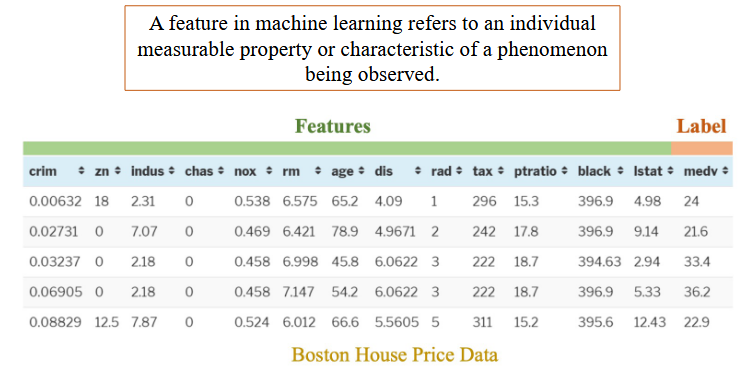
\includegraphics[width=0.8\linewidth]{images/whatfeasture.png}
    \caption{Định nghĩa Feature và Label.}
\end{figure}

\textbf{Feature Store} ra đời để giải quyết hai vấn đề chính:
\begin{enumerate}
    \item \textbf{Vấn đề Kỹ thuật (Training-Serving Skew):} Nó hoạt động như một nền tảng trung tâm, cung cấp một nguồn dữ liệu đặc trưng \textit{duy nhất} cho cả hai môi trường. Logic tính toán đặc trưng được định nghĩa một lần và tái sử dụng, đảm bảo tính nhất quán tuyệt đối.
    \item \textbf{Vấn đề Tổ chức (Hợp tác):} Thay vì mỗi nhóm tự xây dựng lại đặc trưng từ đầu (gây lãng phí tài nguyên), Feature Store cung cấp một "danh mục" (catalog) chung cho phép các nhóm khám phá, chia sẻ và tái sử dụng các đặc trưng đã có.
\end{enumerate}

\subsubsection{Các thành phần cốt lõi của Feature Store}
Một Feature Store hoàn chỉnh bao gồm 5 thành phần chính:

\begin{itemize}
    \item \textbf{Serving (Phục vụ):} Đây là lớp giao diện cung cấp dữ liệu cho mô hình.
    \begin{itemize}
        \item \textbf{Offline Serving:} Cung cấp dữ liệu lịch sử cho \textit{Model Training} (huấn luyện). Dữ liệu này được dùng để huấn luyện lại mô hình theo lịch (ví dụ: hàng ngày) hoặc khi phát hiện data drift.
        \item \textbf{Online Serving:} Cung cấp dự đoán thời gian thực cho \textit{Model Serving} (dự đoán), đảm bảo độ trễ thấp và khả năng mở rộng.
    \end{itemize}
\end{itemize}
\begin{figure}[H]
    \centering
    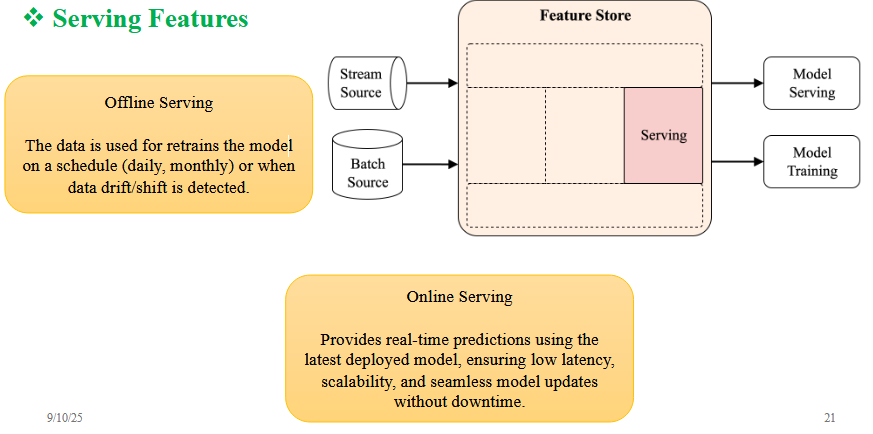
\includegraphics[width=0.7\linewidth]{images/servingfeast.png}
    \caption{Hai chế độ Serving: Offline (cho Training) và Online (cho Serving).}
\end{figure}

\begin{itemize}
    \item \textbf{Storage (Lưu trữ):} Lớp này trừu tượng hóa việc lưu trữ, chia làm hai kho:
    \begin{itemize}
        \item \textbf{Offline Store:} Lưu trữ toàn bộ dữ liệu lịch sử của đặc trưng (có thể là hàng tháng, hàng năm) để huấn luyện. Thường là Data Warehouse (BigQuery, Snowflake) hoặc Data Lake (S3).
        \item \textbf{Online Store:} Chỉ lưu trữ giá trị \textit{mới nhất} của đặc trưng. Được tối ưu cho việc truy vấn tốc độ cao, độ trễ thấp (ví dụ: Redis, DynamoDB).
    \end{itemize}
\end{itemize}
\begin{figure}[H]
    \centering
    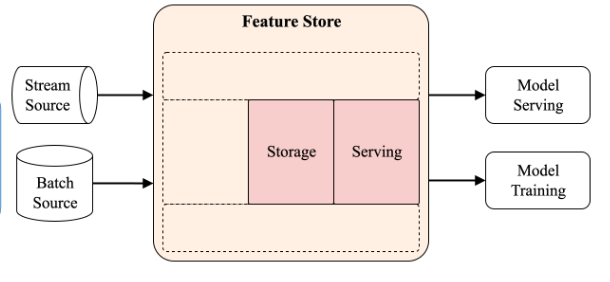
\includegraphics[width=0.7\linewidth]{images/storage_feast.png}
    \caption{Hai thành phần lưu trữ: Offline Store và Online Store.}
\end{figure}

\begin{itemize}
    \item \textbf{Transformation (Biến đổi):} Quản lý và điều phối các tác vụ tính toán đặc trưng từ dữ liệu thô.
\end{itemize}
\begin{figure}[H]
    \centering
    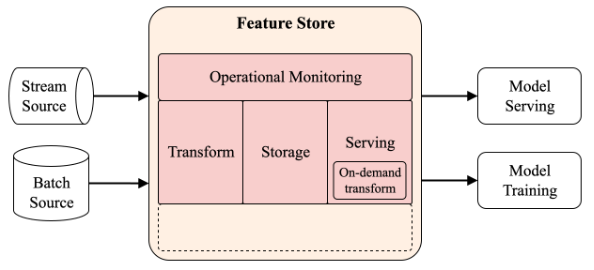
\includegraphics[width=0.7\linewidth]{images/transform_feast.png}
    \caption{Lớp Transformation, Storage, Serving và Monitoring.}
\end{figure}

\begin{itemize}
    \item \textbf{Monitoring (Giám sát):} Theo dõi sức khỏe của hệ thống. Quan trọng nhất là giám sát "data drift" (sự thay đổi trong phân phối thống kê của dữ liệu) và phát hiện "training-serving skew".
\end{itemize}
\begin{figure}[H]
    \centering
    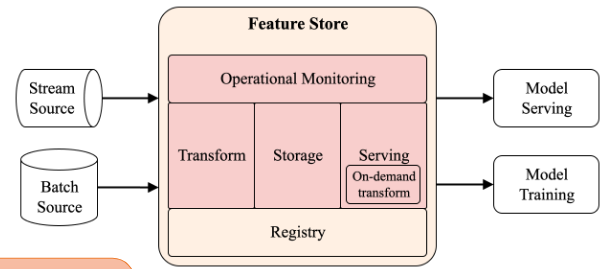
\includegraphics[width=0.7\linewidth]{images/monitor_feast.png}
    \caption{Lớp Monitoring giám sát chất lượng dữ liệu và vận hành.}
\end{figure}

\begin{itemize}
    \item \textbf{Registry (Sổ đăng ký):} Là bộ não của Feature Store. Đây là thành phần trung tâm, đóng vai trò là "nguồn chân lý duy nhất" (single source of truth) lưu trữ mọi định nghĩa, siêu dữ liệu (metadata) về các đặc trưng.
\end{itemize}
\begin{figure}[H]
    \centering
    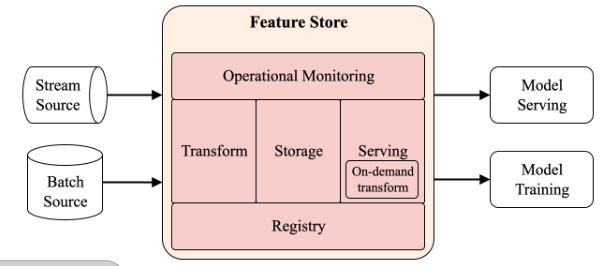
\includegraphics[width=0.7\linewidth]{images/registry_features.png}
    \caption{Registry là thành phần trung tâm lưu trữ mọi định nghĩa.}
\end{figure}

\subsubsection{Lợi ích của Feature Store}
Trong bối cảnh bài toán gian lận, việc áp dụng Feature Store mang lại các lợi ích rõ rệt:
\begin{itemize}
    \item \textbf{Đảm bảo tính nhất quán:} Giải quyết triệt để Training-Serving Skew bằng cách đảm bảo tính nhất quán giữa dữ liệu huấn luyện (training) và dữ liệu dự đoán (inference).
    \item \textbf{Tăng tốc độ phát triển:} Cho phép theo dõi và chia sẻ đặc trưng giữa các nhà khoa học dữ liệu thông qua một kho lưu trữ có phiên bản.
    \item \textbf{Phục vụ đa mục đích:} Cung cấp đặc trưng cho nhiều trường hợp sử dụng ML: huấn luyện mô hình, xử lý theo lô, và dự đoán thời gian thực.
    \item \textbf{Giám sát chất lượng dữ liệu:} Giám sát chất lượng dữ liệu để nhanh chóng xác định các lỗi pipeline hoặc "data drift".
\end{itemize}

\subsection{Feast là gì?}

\begin{figure}[H]
    \centering
    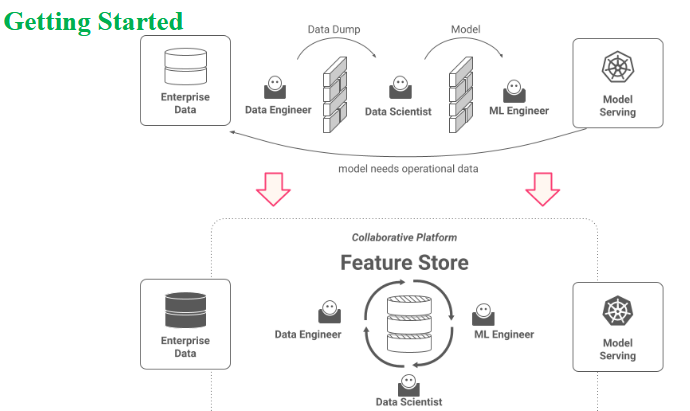
\includegraphics[width=0.9\linewidth]{images/whyfeast.png}
    \caption{Triết lý của Feature Store: Chuyển từ quy trình riêng rẽ (trên) sang nền tảng hợp tác (dưới).}
\end{figure}

Như trong hình, quy trình truyền thống (ở trên) thường bị "vỡ": Kỹ sư dữ liệu (Data Engineer) thực hiện "Data Dump", trong khi Nhà khoa học dữ liệu (Data Scientist) và Kỹ sư ML (ML Engineer) làm việc riêng rẽ trên dữ liệu của họ. Tạo ra 1 bức tường ngăn cách phối hợp giữa 2 nhóm. \\

Feature Store (ở dưới) phá vỡ các bức tường này, tạo ra một \textbf{Nền tảng Hợp tác (Collaborative Platform)}, nơi tất cả các vai trò cùng tương tác với một kho lưu trữ đặc trưng duy nhất. \\

\textbf{Feast} là một Feature Store. Triết lý cốt lõi của Feast là nó \textbf{không phải là một nền tảng "tất cả trong một"}. Thay vào đó, nó được thiết kế như một \textbf{lớp điều phối mỏng và linh hoạt}, với mục đích kết nối và tái sử dụng hạ tầng dữ liệu mà tổ chức của bạn \textit{đã có sẵn}.
\begin{itemize}
    \item Feast \textbf{không} thay thế Data Warehouse (như Snowflake, BigQuery) $\rightarrow$ nó \textbf{sử dụng} chúng làm \textit{Offline Store}.
    \item Feast \textbf{không} thay thế CSDL Key-Value (như Redis) $\rightarrow$ nó \textbf{sử dụng} chúng làm \textit{Online Store}.
\end{itemize}

\subsubsection{Kiến trúc và các thành phần của Feast}

\begin{figure}[H]
    \centering
    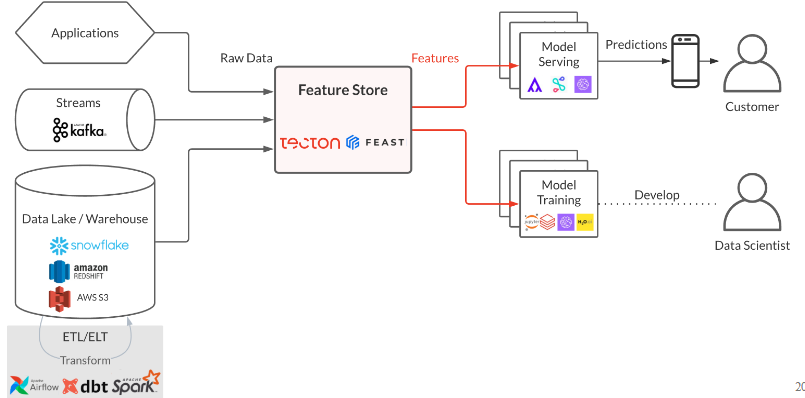
\includegraphics[width=\linewidth]{images/feast_pipeline.png}
    \caption{Kiến trúc tổng quan của Feast trong MLOps.}
\end{figure}

Kiến trúc của Feast thể hiện rõ triết lý của nó. Feast đóng vai trò trung tâm, tiếp nhận dữ liệu thô (Raw Data) từ nhiều nguồn đầu vào:
\begin{itemize}
    \item \textbf{Data Lake / Warehouse} (ví dụ: Snowflake, Amazon Redshift, S3).
    \item \textbf{Streams} (ví dụ: Kafka).
    \item \textbf{Applications} (các ứng dụng nghiệp vụ).
\end{itemize}

Sau đó, Feast quản lý và phục vụ các Đặc trưng (Features) này cho hai đích đến:
\begin{enumerate}
    \item \textbf{Model Training (Huấn luyện):} Cung cấp dữ liệu lịch sử (offline) cho các Nhà khoa học dữ liệu (Data Scientist) để phát triển (Develop) mô hình.
    \item \textbf{Model Serving (Phục vụ):} Cung cấp dữ liệu (online) cho các mô hình đã triển khai để đưa ra dự đoán (Predictions) cho Khách hàng (Customer).
\end{enumerate}

Để thực hiện điều này, Feast sử dụng các thành phần tương tự như một Feature Store lý thuyết, nhưng với các định nghĩa cụ thể:

\begin{itemize}
    \item \textbf{Storage (Offline/Online Store):} Như đã nói, Feast \textit{sử dụng} hạ tầng có sẵn của bạn. Trong file cấu hình, bạn sẽ chỉ định `offline\_store` (ví dụ: một file Parquet, một bảng BigQuery) và `online\_store` (ví dụ: Redis, SQLite).

    \item \textbf{Serving (Offline/Online Serving):} Feast cung cấp hai hàm SDK chính để truy vấn dữ liệu:
    \begin{itemize}
        \item `store.get\_historical\_features(...)`: Dùng để truy vấn \textbf{Offline Store}. Hàm này thực hiện các phép join \textit{point-in-time correct} (chính xác tại thời điểm) để chống rò rỉ dữ liệu khi huấn luyện.
        \item `store.get\_online\_features(...)`: Dùng để truy vấn \textbf{Online Store}. Hàm này lấy vector đặc trưng mới nhất với độ trễ thấp nhất cho việc dự đoán thời gian thực.
    \end{itemize}

    \item \textbf{Registry (Sổ đăng ký):} Đây là trái tim của Feast. Thay vì là một khái niệm trừu tượng, trong Feast, đây là một \textbf{feature repository} (kho chứa đặc trưng) mà bạn định nghĩa bằng code Python. Bạn sẽ khai báo các đối tượng như:
    \begin{itemize}
        \item \textbf{DataSource:} Nơi dữ liệu của bạn được lưu trữ (ví dụ: file Parquet).
        \item \textbf{Entity:} Đối tượng kinh doanh mà bạn muốn mô tả (ví dụ: `customer\_id` hoặc `transaction\_id`).
        \item \textbf{FeatureView:} Một nhóm logic các đặc trưng được liên kết với một Entity và một DataSource.
    \end{itemize}
    Khi bạn chạy lệnh `feast apply`, các định nghĩa Python này sẽ được đăng ký vào file `registry.db`.
\end{itemize}


\section{Phần 4: Case Study}


\section{Phần 5: Final Revision: ôn lại mọi khái niệm trong bài cùng team Time Series}


\printbibliography % Bỏ comment dòng này nếu bạn có tệp .bib

\end{document}
